\section{Modular approach in manipulation}
\label{cha4:sec2}


This section presents the method we used to modularize human demonstration of manipulation tasks. Our goal is to acquire a modular based control policy for an object manipulation task from human demonstration. To this end, we take a three-step approach:
\begin{enumerate}
\item Human demonstrating a task in different contexts (Section~\ref{cha4:sec2:demo}).
\item Extracting human control strategies for different contexts and build multiple internal models(Section~\ref{cha4:sec2:learn}).
\item Use the multiple models to compute motor commands for a robot(Section~\ref{cha4:sec2:control}).
\end{enumerate}

Figure~\ref{fig:overview} shows an overview of our framework.

\begin{figure}
  \centering
   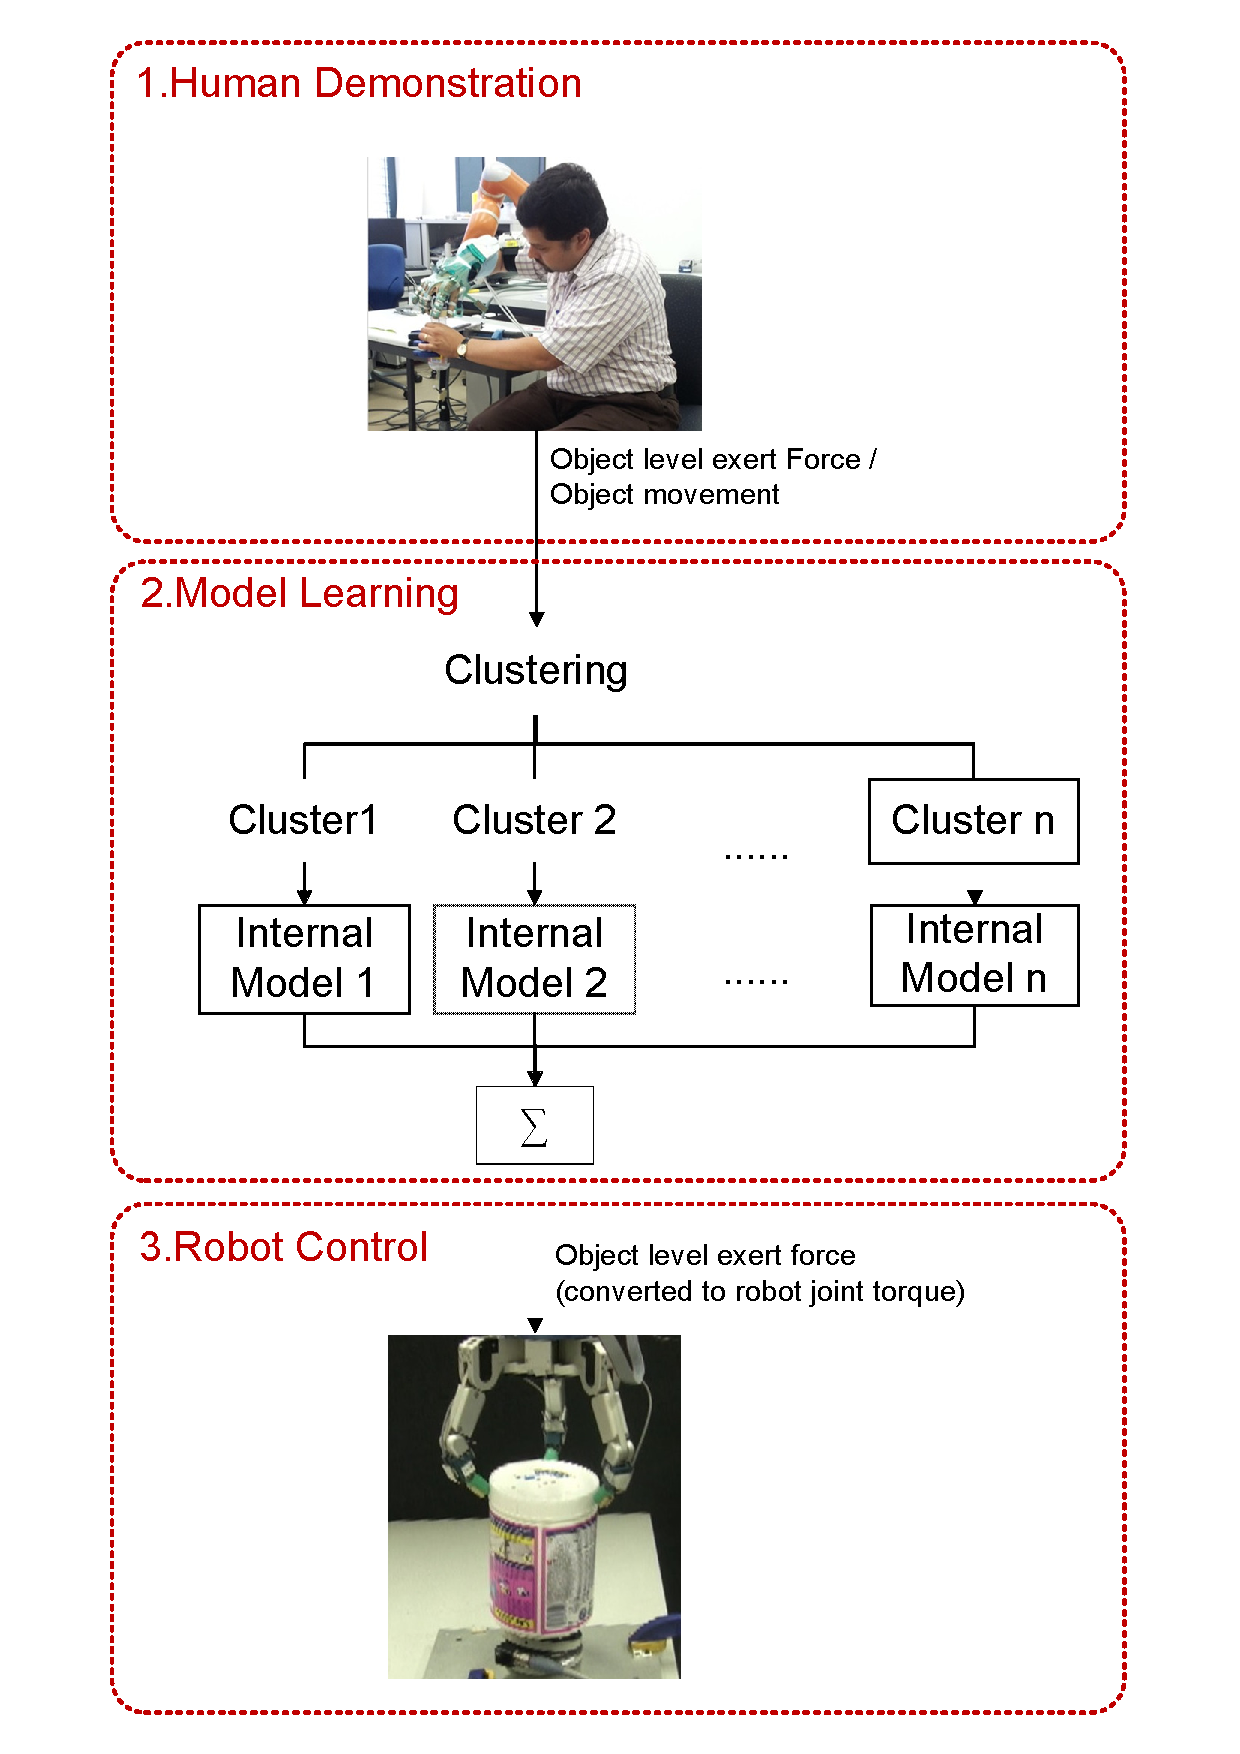
\includegraphics[width=15cm]{./fig_cha4/overview3.pdf}
  \caption{ \scriptsize{System overview.}
  \label{fig:overview}
}
\label{fig:demo}
\end{figure}

\subsection{Human demonstrating tasks with direct contact to objects}
\label{cha4:sec2:demo}


\begin{figure*}
  \centering
    \subfloat[\scriptsize{Optitrack markers attaching to a cap}] {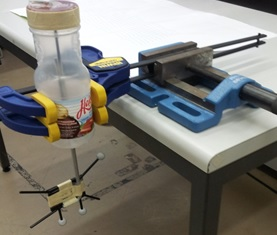
\includegraphics[height=4cm]{./fig_cha4/marker2.jpg}}
    \subfloat[\scriptsize{Force torque sensor}] {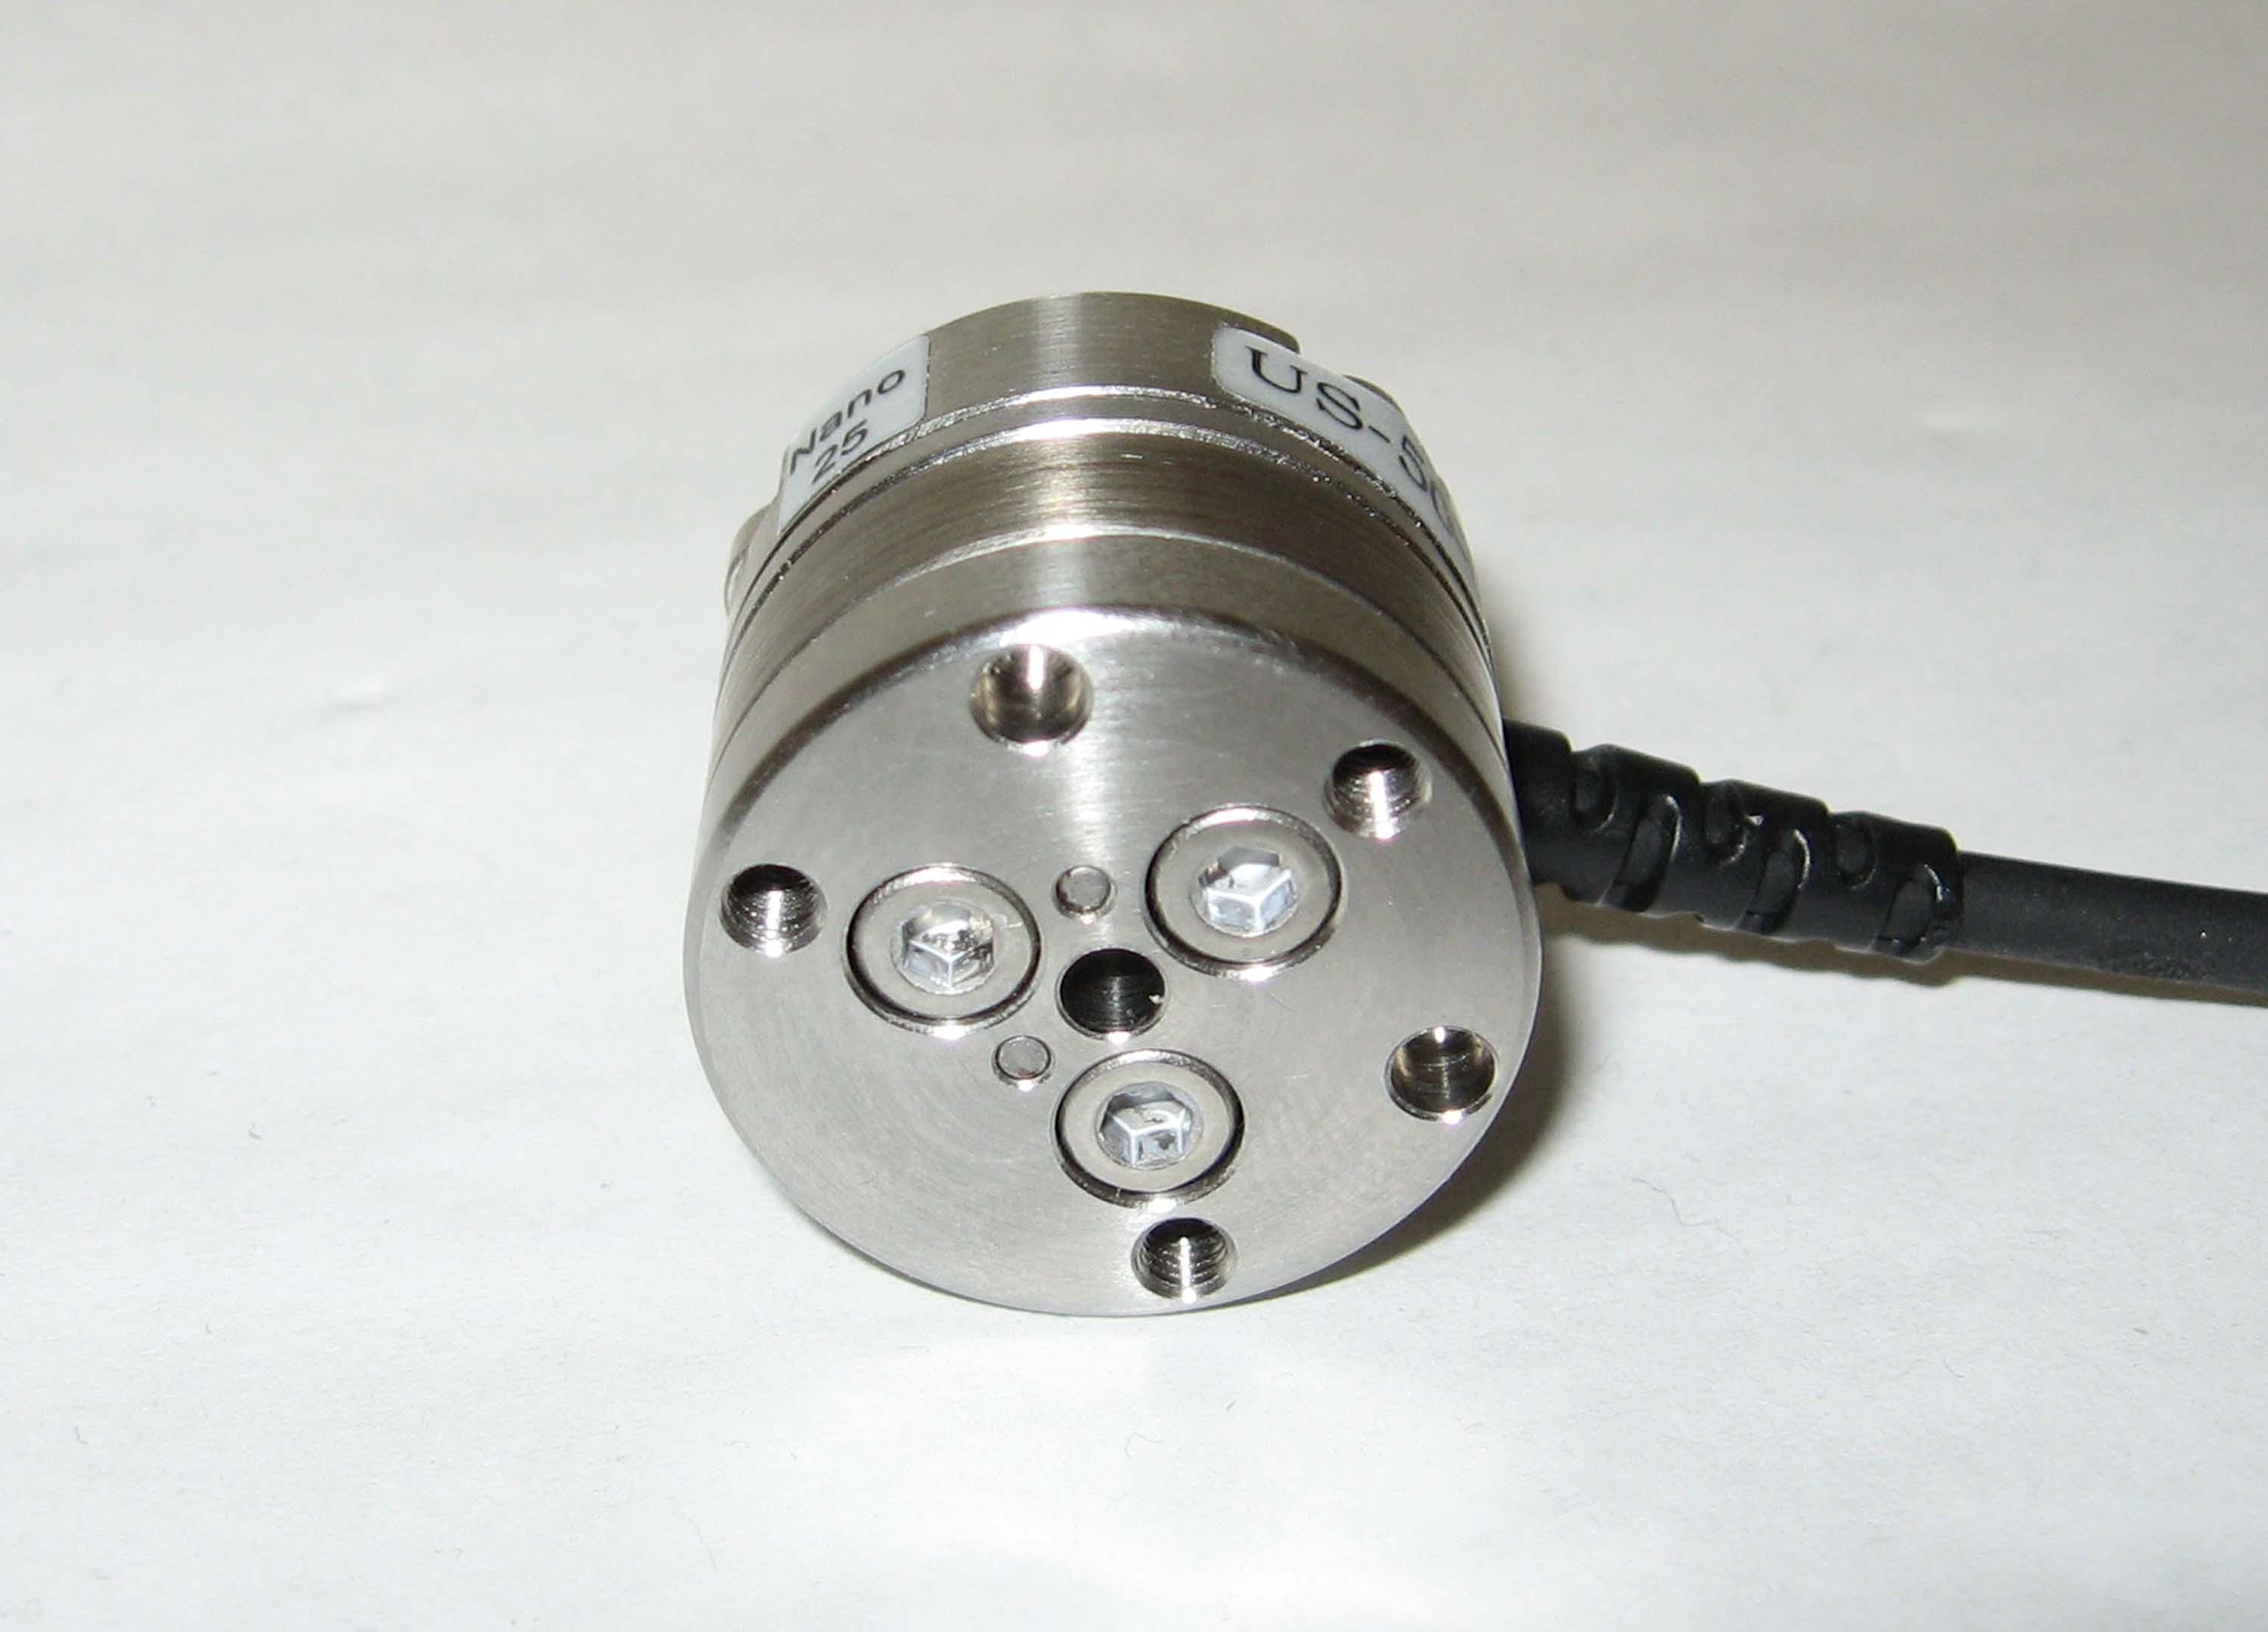
\includegraphics[height=4cm]{./fig_cha4/Nano25-E.jpg}}
    \subfloat[\scriptsize{Texscan tactile sensors mounting to a glove}] {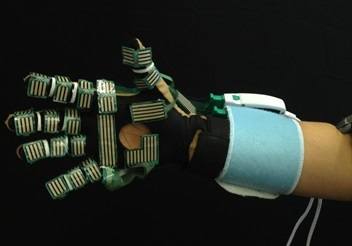
\includegraphics[height=4cm]{./fig_cha4/texscan2.jpg}}
    \caption{\scriptsize{Sensors used in the human demonstration of opening a bottle cap task.}}
  \label{fig:devices}
\end{figure*}

%Learning manipulation tasks is one of the main application of this approach. The physical properties of a manipulation task is hard to express analytically, and as a result the control strategy is hard to derive. Modeling expert's demonstration of strategies has been used as an alternative to the analytical solution.

The first step is to demonstrate a task to a robot. Two major forms of demonstration are used in teaching manipulation tasks: kinematics teaching and tele-operation.

\paragraph{Kinematics teaching} ~\\
% ===== Why not kinematics approach? =====
In kinesthetic teaching, human directly contact with the robot and guide their movements to accomplish a task~\cite{korkinof2013online,pais2014encoding,pastor2011skill,Miao2014}. The trajectory of movements and contact force are recorded by the robot sensors.
This method is simple and effective but limited in the number of controllable end effectors. While a manipulation task usually involves multifinger movement, a human can kinematically operate one finger with each hand and hence two fingers simultaneously at most. Hence kinesthetic teaching is not feasible for demonstrating multifinger task.

\paragraph{Tele-operation teaching} ~\\
To control multi-finger hands, some researchers use tele-operation~\cite{bernardino2013precision,kondo2008recognition,Fischer98}. This usually relies on data gloves to sense hand posture, and motion capture system to sense human hand-arm motions. The human motion is mapped to robots to generate motions and interact with the environment. In fine manipulation tasks, the robot platforms are usually restricted to anthropomorphic hands for better mapping. All of the above methods provide no direct force feedback to the human demonstrator during manipulation.

\paragraph{Human direct demonstration} ~\\
In some studies, the human demonstrate manipulation tasks with their own bodies~\cite{asfour2008imitation}. With direct interaction with the object, human is able to perform the task most naturally and with a more delicate control strategy. The task information captured from these human demonstrations needs to be transferred to robots. Because the difference of the embodiment between human and robot, a mapping between them has to been built. Various mapping methods have been proposed~\cite{do2011towards,asfour2008imitation,hueser2006learning}, while human correction~\cite{calinon2007incremental,sauser2011iterative,romano2011human} and self-correction via learning~\cite{bidan2013robio} are proposed as alternative solutions. These methods are quite robot specific or task specific. In general, how to effectively transfer human skills to robots skill remains a open problem.

Here We use a method to allows the subject to perform natural feedback control strategies in demonstration, while the strategy can then be easily transfer to any robot platform. In our task demonstrations, a human wears tactile sensors and directly interacts with objects. In this way, human demonstrator have direct cutaneous and kinaesthetic feedback, which is desirable for good manipulation demonstration. To make the information embedded in the demonstration can be easily transfer to robot, the demonstration is expressed from an ``object centric viewpoint''.


%============= Object Centric =============
\paragraph{Object centric representation} ~\\
The object centric viewpoint considers a manipulation task from the object's perspective, which suggests the goal of learning a manipulation task is to reproduce the same object behavior, rather than reproduce the demonstrator's movement. This makes sense as human may use different ways to accomplish a manipulation task: the motion or posture might be different but the effect on the object is the same. What the robot needs to imitate is the effect on the object but not the movements.
Hence our approach takes this principle and learns a control strategy to produce a desired object behavior, rather than to produce a human or robot behavior. This strategy expressed from the object perspective can be transfer to a robot platform by covering the exert force to robot joints' torque with Jacobian matrix. From the object centric viewpoint a manipulation problem is simplified: we transfer from a problem of controlling multifinger (multi-endeffector) and its impact of the environment to controlling an object.

Based on the object centric principle, we collect the object trajectory and its driven force. These data can be accessed by motion capture system, force-torque sensor and wearable haptic device. Fig.~\ref{fig:devices} shows a few sensors we used in the opening bottle caps task. The representation of data will be explained in Section~\ref{cha4:sec2:learn:objectlevel}


% ======= demonstrate in different context   =======
\paragraph{Demonstrations in different task contexts}  ~\\
During the demonstrations, the teacher perform a task a number of times to generate enough data for capturing the key features. Further, the teacher perform the task under different system kinematics and dynamics configurations, e.g. friction conditions, in order to explore how human adapt to different task contexts. These different configurations are chosen to cover a wide range of different contexts. These wide range demonstrations are then used to learn a multiple module model.





\subsection{Learning a Multiple-Module Model}
\label{cha4:sec2:learn}
In this section we detail our modeling method, explaining why do we use modular approach and how do we model human manipulation strategy.

%% Internal model
%In the study of human motor control, internal model is one of the most evidently supported hypothesis. It postulates a neuron process that simulates output of the motor system and the environment~\cite{kawato1999internal}. It's applications in robot control have been explored by many researchers. Various types of internal models are built for different tasks~\cite{sciavicco2000modelling,jordan1992forward}.

% Adaptive
Modular approach is used in adaptive control and its benefit has been long discussed~\cite{jacobs1991adaptive,narendra1997adaptive}.
In manipulation tasks, context changing is a common phenomenon due to object interactions. These changes are often rapid or discontinuous. Classic adaptive control approaches such as model identification~\cite{khalil2004modeling} are inadequate for these tasks, as instability or error may occur during the optimization of the model variables. To fast adapt, the multiple model approach~\cite{narendra1995adaptation}, referred as modular approach here, is proposed. In this approach, multiple controllers are designed, each of which in charge of a certain task context. During control, the task context is estimated online and the corresponding controllers are activated.  Some recent work~\cite{fekri2007robust,kuipers2010multiple,sugimoto2012emosaic} presents promising modular based approaches.

% Modular - human MOSAIC

%%The excellent ability of human to manipulate different objects in different contexts and to quickly adapt to change of contexts suggested that our central nervous system (CNS) maintains multiple internal models            of outside environments, rather than a single internal model that adapts to new environment~\cite{neilson1985acquisition}.
%Based on the concept of modularity, the Modular selection and identification for control (MOSAIC) architecture was proposed to explain the motor control strategy of the CNS~\cite{wolpert1998multiple}. According to this hypothesis, during the motor control process, the brain quickly select the most appropriate modules according to the current environment context and use them to generate an appropriate motor command to react to the environment~\cite{haruno2001mosaic}.

% Our approach
The excellent ability of human to manipulate different objects in different contexts and to quickly adapt to change of contexts suggested that our central nervous system (CNS) maintains multiple internal models of outside environments, rather than a single internal model that adapts to new environment~\cite{neilson1985acquisition}. Indeed, neuroscience evidence suggests that animal brain sum modular stimulates of muscles to generate different motions~\cite{mussa1994linear}. Inspired by this, we take a modular approach to model human adaptive control strategy.



\paragraph{Our modular strategy} ~\\
The modular approach we take is inspired from MOSAIC (Modular selection and identification for control)~\cite{haruno2001mosaic}, one of the pervasive multiple module models for human motor control mechanism.

The system of MOSAIC is constituted by multiple parallel modules. Each module has three components: a forward model, an inverse model and a responsibility factor (RF). The forward model is responsible for estimating the task context in real time, and the inverse model is used to generate appropriate motor command for the context. These two models are connected by the RF. The task context estimated by the forward model is compared with the actual current task context.
The RF of each module is computed according to the accuracy of the estimation: the more accurate the forward model predicts, the higher the RF is (detailed in Section~\ref{cha4:sec2:control:rf}). The RF of all modules are computed and then normalized.
The inverse models are weighed by its normalized RF. The final motor command is the linear combination of the commands factored by their weighs. With this mechanism, the module predicting the current task context better takes more responsibility in the final motor command. Figure~\ref{fig:control} sketches the work flow of this system. Though the MOSAIC has gained a large concerns in neuroscience community, this approach is not widely used in robot control.

We take this paradigm and model our internal models by GMM. Training GMM with the Expectation Maximization algorithm (EM), we estimate the optimal values of the model parameters. Compare to the early work~\cite{wolpert1998multiple} which use Neural Network and has to manually tune the variance of each forward model, GMM has the advantage of automatically computing the all the model parameters. Later work~\cite{haruno2001mosaic} fixes the hand tuning problem by modeling with Hidden Markov Model (HMM) and optimize the model with EM. With this method the forward models are assumed to be linear. In our approach, GMM allows non-linear system to be modeled. Fig.~\ref{fig:control} illustrates the workflow of our approach. Compare to the switching modular method~\cite{narendra1997adaptive}, i.e. only one module will be activated and used to generate motor command, the linear combination of the modules requires less number of modules to approximate the system dynamics.

In some tasks the forward model and inverse model are united to a single model~\cite{petkos2006learning}. For that particular task the action ($a_t$) taking the current task state ($s_t$) to the desired task state ($s_{t+1}$) is always unique. However, in many cases this mapping is not unique and hence the inverse model has to include extra variables in order to resolve the non-uniqueness. In our approach we build the forward and inverse model separately.
%However this model does not provide a method to find out number of models needed in tasks. %and the inverse model represented by the joint distribution will potentially produce an invalid command that average all possible solutions.

Despite the many applications and discussions of the modular approach, how to systematically modularize the control strategy presented during the human demonstration, i.e. determine the number of modules and build appropriate model for each module, still remains a open problem. We tackle this problem by a data driven approach. We cluster the demonstration data with an hierarchical approach and model each cluster as a pair of forward and inverse model. This solution can be applied to modularize many manipulation tasks. A similar clustering method has been applied to group and build tree structure of human motion pattern primitives~\cite{kulic2008incremental}. To cluster the motion primitives, a high value and a low value of the cut off parameter are tested to evaluate the trade off effect between facilitating quick tree formation and introducing misclassification. In our approach, the cut off parameter is determined by the variance of the data and hence avoid this step. This provide us with a proper grouping of the data and which can generate proper motor command for control. To the best of our knowledge, our work is the first realization of the modular approach in learning an object manipulation task with a real robot.

%
%
%Scientist has long been fascinated by human adaptive motor control ability and wondering the mechanism of it. One of the most evidently supported hypothesis is the multiple model~\cite{neilson1985acquisition}. %~\cite{haruno2001mosaic}



\subsubsection{Object centric manipulation strategy}
\label{cha4:sec2:learn:objectlevel}


As mentioned in Section~\ref{cha4:sec2:demo}, one of the challenges in imitation learning is the mapping problem, i.e. how to map the teacher's motions to the robot's motions so that they produce the same effects. This mapping becomes more difficult for object manipulation tasks, the goal of which is to deliver the object from the current state to a desired state. During this process the movement of the manipulator is bounded not only by its own kinematic constraints but also bounded by by the movement of the object. It is more important to imitate how human apply forces to achieve object's desired movement, than to imitate the human limb movement.
Therefore we take an ``object centric approach"~\cite{okamura2000overview}, of which the control policy is taken from the object point of view.


Therefore, our model encodes a force and torque profile rather than the end effector movement trajectory. The imitation learning objective here is not to find a policy for the end effector movement but to find a policy that maps the force and torque to the object movement. This policy allows the robot to efficiently acquire new behaviors to accomplish the task. %Different robots move differently to achieve the desired object movements.
Giving the robots' kinematics and the desired exert force on the object, the joint torques can be deduced by the Jacobian matrix~\cite{okamura2000overview}. To this end, we focus on the force-torque-displacement tuple: $\{F,\tau,s\}$ demonstrated in the task. In later sections, we refer $\{F,\tau\}$ as the motor command with notation $\{a\}$. In each demonstration, a time series of the tuple is recorded.



\subsubsection{Decide number of modules}
\label{cha4:sec2:learn:cluster}

% ----------- why clustering -----------
Due to object interaction, a manipulation task frequently encounter abrupt changes of the system dynamics, e.g. transfer between statuses with no contact and with contact, between statuses driven by static friction and by driven dynamic friction. Different strategies should be used to handle different dynamics and hence a multiple module model is desired. Our approach is to extract different strategies from demonstration and build one module for each of the strategies. During implementation, the system can quickly estimate the context by the sensory inputs and weight the modules according to their reliability and then generate a contextilize motor command.

% ---------- Cluster to find number of modules -----------
Different tasks may need different number of modules. This number may not be easy to find. In previous studies~\cite{sugimoto2012emosaic,haruno2001mosaic}, the number of modules is defined as number of different target objects or different phases in the task, which can be clearly distinct such as no load or on load. However this is not always the case. In a task involve more phases, human may regard different phases as the same task context and handle them with the same control strategies. A recent study suggests that modularize a control strategy by the number of objects can cause redundancy of modules and hence is inefficient~\cite{lallee2009}.

Here we propose a data-driven approach to properly define the number of modules for a given task.
To this end, we should differentiate different types of strategies. The differences can be reflected from the different patterns of the force-torque-displacement tuple. We differentiate the patterns by clustering. Data in the same cluster is considered to be governed by the same strategy. The number of clusters is the number of modules and each module is encoded by one model.


% ----------- Distance Metric for clustering ------------
The goal of clustering is to separate a set of data to a few groups according to their similarities, such that the data in the same group are more similar to each other than those in different groups. This technique has very important applications in computer vision and language processing~\cite{warren2005clustering}. Numerous clustering algorithms have been proposed for different purposes.

Before clustering, we need to measure the similarities, i.e. the distances, between the data points we want to cluster. The similarity metric is user defined according to the purpose of clustering. One of the mostly used metric is the Euclidean distance. Different from an usual clustering problem, however, the data we need to cluster are not a set of single data points but a set of time series. Each time series include a sequence of data point. Here we use the Dynamic Time Warping technique (DTW) to measure the distance between each pair of time series~\cite{berndt1994using}.

\paragraph{Dynamic time warping} ~\\
%%%%%%%%%% TODO: DTW explaination, citation.
Dynamic time warping is a technique for measuring the similarity between two time series, which may have different speeds or durations. It has an important application in speech recognition. For example, two person may speak the word ``hello''in different speeds. By the DTW, one is able to tell they are speaking the same word. This is achieved by warping the single in the time dimension. The two time series are ``aligned'' by finding their optimal match. The similarity is computed as the average distance between the corresponding points of the two time series. By this method, the similarity computed by DTW is independent to the variance in the time dimension. Figure~\ref{fig:alignDTW} shows an example of alignment of two time series by DTW.

Here we make an assumption that our manipulation task is time independent, i.e. in the time scale, whenever we apply the same force we will achieve the same state. This assumption is feasible for a large range of tasks.

\begin{figure}
  \centering
  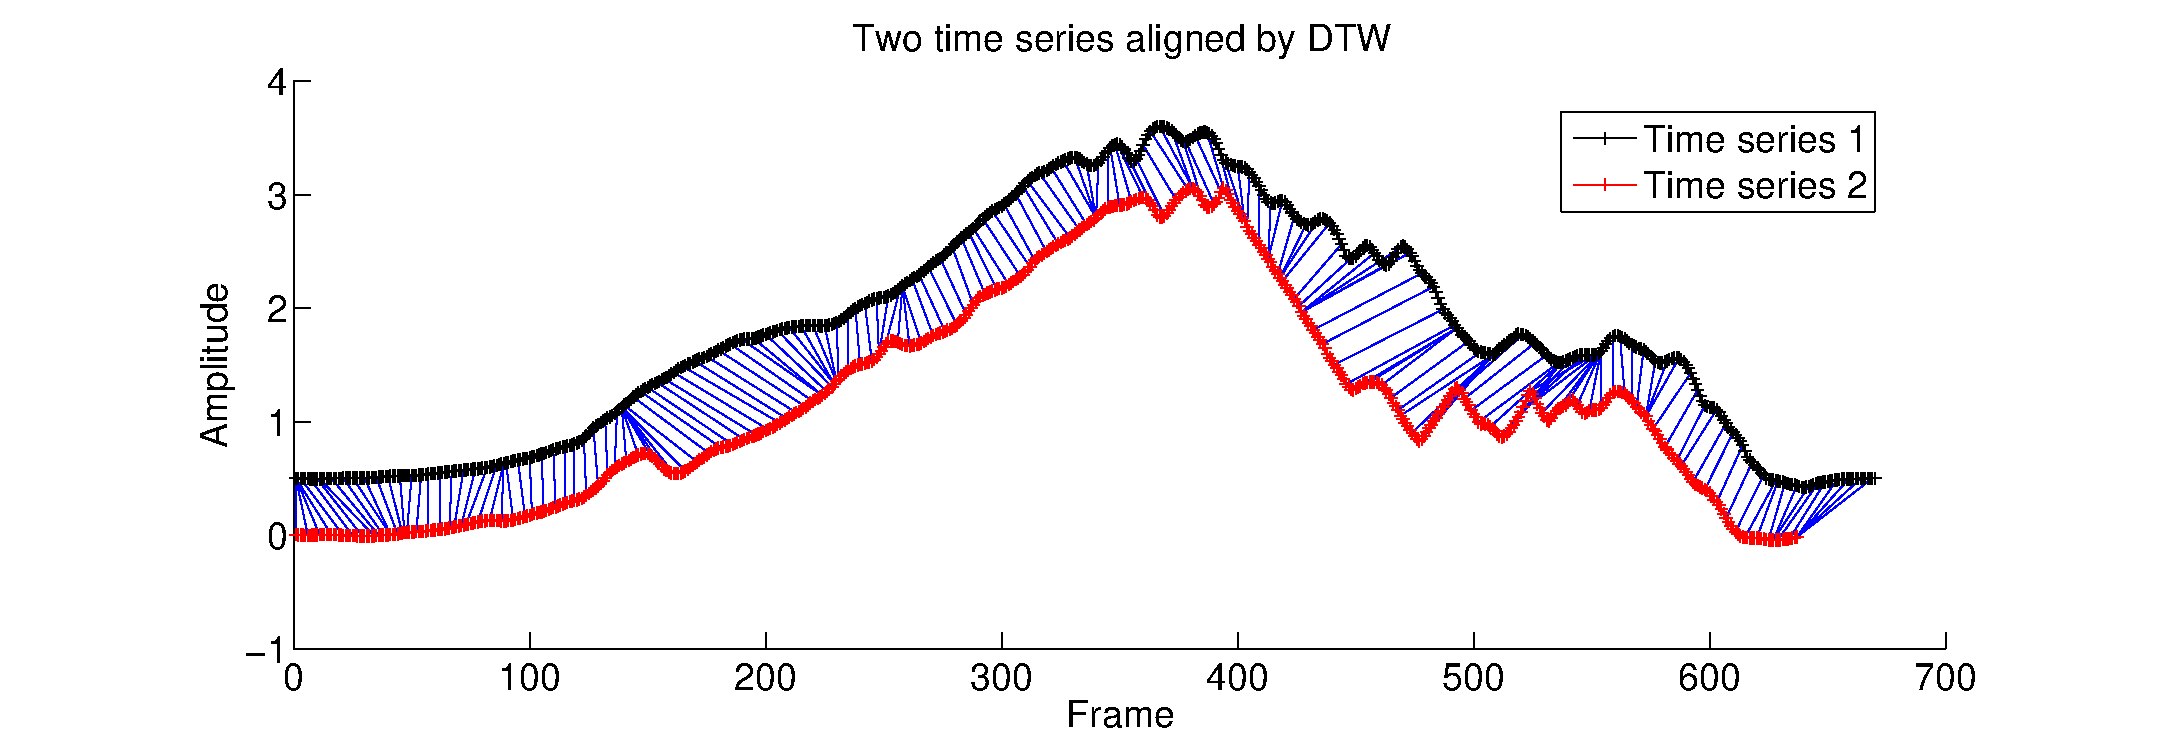
\includegraphics[width=16cm]{./fig_cha4/alignDTW.eps}
  \caption{ \scriptsize{Two time series aligned by DTW. Red and black lines are the raw time single. The blue lines connect the matching points between them. DTW wrap the two time series nonlinearly so that the time independence similarity can be measured. The time series 1 is moved up by 0.5 for display reason.}
}
\label{fig:alignDTW}
\end{figure}



\paragraph{Grouping data} ~\\
Two of the most dominate clustering methods are k-means clustering and hierarchical clustering. K-means is a centroid based grouping method. Given the number of clusters k, it find a way to group the data such that the sum of distance from each point to its belonging group center is minimized. Hierarchical clustering is a connectivity based method. There are two types of hierarchical clustering method: agglomerative and divisive. Here we focus on the agglomerative method as it is more widely used. The hierarchical clustering method groups similar data iteratively. At the beginning each data point is a single cluster. In each iteration, two most similar clusters are merged to one. This step repeats until a stop criteria is satisfied or all data is merged to one cluster. Usually the merges are done in a greedy manner and hence no optimization is needed. Figure~\ref{fig:hcluster} illustrates the principle of hierarchical clustering. This clustering algorithm does not require to know the number of clusters beforehand.

%% ------------ Hierarchical clustering -----------
In our case, the number of clusters is an unknown variable. Therefore we use the hierarchical (agglomerative) clustering method~\cite{willett1988recent} to group our data. The similarity (distance) between each pair of time series is computed by DTW. This produces a distance matrix. Each element in the matrix is the distance between two time series a and b, where a and b are the row and column index of the element. At the beginning of clustering, each time series is a single cluster. The distance between each cluster is read from the distance matrix. After one iteration, clusters are merged and most new clusters contain more than one times series. The distance between the new clusters is computed by the average distance between a member of one cluster to a member of the other cluster (average linkage).

\begin{figure}
  \centering
   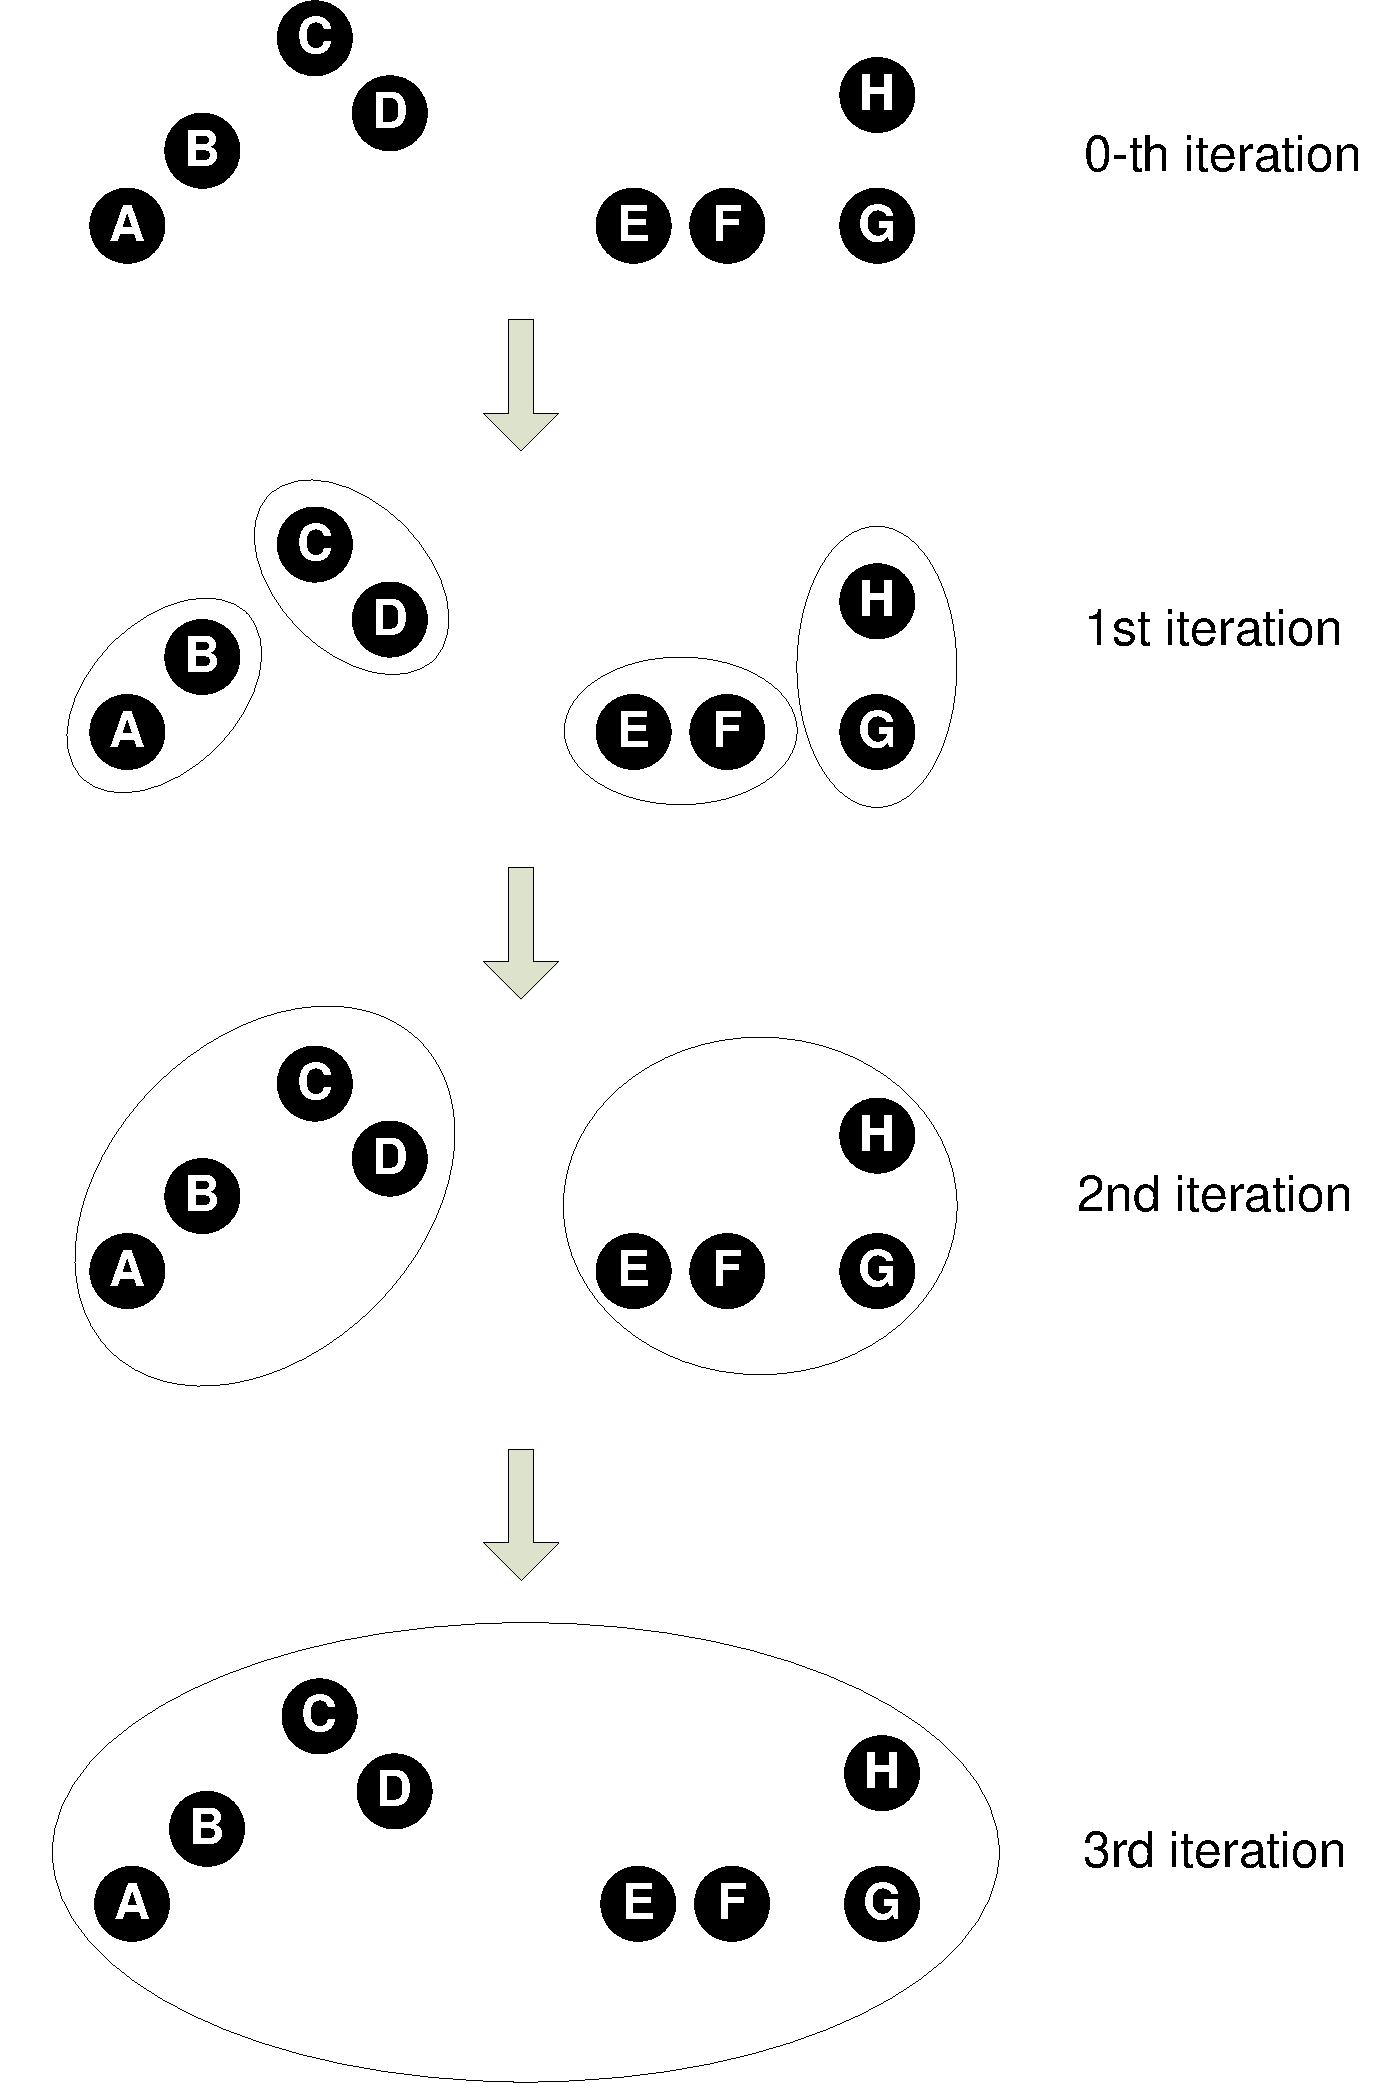
\includegraphics[width=12cm]{./fig_cha4/hierarchicalclustering.pdf}
  \caption{ \scriptsize{A sketch of the hierarchical agglomerative clustering method. The nearest two clusters are grouped into one at each iteration until a single cluster is formed.}
}
\label{fig:hcluster}
\end{figure}

Our hierarchical clustering method has one more constraint: the threshold of distance. Two clusters can be merged to one only when their distance is smaller than the threshold. This threshold is set by the variance of the data from the same setup. As mentioned above (Section~\ref{cha4:sec2:demo}), a task is demonstrated a few times under the same setup. These demonstrations are presumed to be handled with the same strategy and hence belong to the same cluster. The variance of these demonstrations gives a reference of the variance of a cluster. The largest variance, across the variance of all setups, is used as the threshold for the clustering. Our clustering method is described as follow:

\begin{enumerate}
\item At the beginning, each single time series is considered to be one cluster.
\item Compute the distances between each pair of clusters.
\item Starting from the first cluster, find its nearest cluster. We define the distance between two clusters to be the average distance across all the time series pairs in them. If the distance to the nearest cluster is smaller than the threshold, merge these two cluster.
\item Move to the next cluster. Repeat the last step for the rest of the clusters.
\item A new set of clusters are formed by the last few steps, move to the next hierarchy and repeat the step 2 to 4 until no new clusters can be formed.
\end{enumerate}

Pseudocode of the complete algorithm is shown in Algorithm~\ref{code:cluster}.

\begin{algorithm}
  \caption{Agglomerative Hierarchical Clustering}
  \begin{algorithmic}[1]
%    \Require{$x$ and $y$ are packed strings of equal length $n$}
%    \Statex Init();
    \State Init(): Make each time series a cluster\;
    \State $mergeable$ = true\;
    \Function{Merge}{all clusters, distance matrix} %      \Comment{$\oplus$: bit}
    \While{mergeable is true}
      \State $mergeable$ = false\;
      \For{each cluster}
        \State $ClusterA$ = current cluster\;
        \State $ClusterB$ = nearest neighbor of $ClusterA$\;
        \If{distance($ClusterA, ClusterB$) $<$ clustering threshold}
            \State Merge $ClusterB$ into $ClusterA$\;
            \State $mergeable$ = true\;
        \EndIf
      \EndFor
      %\State \Return{$\delta$}
    \EndWhile
    \EndFunction
  \end{algorithmic}
  \label{code:cluster}
\end{algorithm}

% --------- Number of cluster -----------
When the clusters can not be merged further, i.e. all clusters are further away from each other than the threshold, we define the number of modules for this task to be the number of the remaining clusters. Each cluster is then modeled as a module. Each module encodes a strategy of handling a specific task context.



\subsubsection{Learning Models}
\label{cha4:sec2:learn:model}

%%%%%%%%%%  TODO: MOSAIC
After identifying the number of modules, we build models for each of the module. In this section, we explain the way we encode human manipulation strategy.

During demonstrations, we constantly acquire the object displacements and the force and torque applied by the teacher. The teacher is the only source of exert force and torque of the system. The relationship between the exert force and torque and their resulting object displacement shows the dynamic characteristic of the task.

%GMM
In our approach, we model the correlation of the force and the displacement with GMM. The task dynamics is hence encoded as a joint distribution of the object status displacement $s$ and the action $a$ taken by human $p(s,a,{\mid}{\Omega})$. In our task, $s$ is the one dimensional cap angular displacement and $a$ is the one dimensional exert torque and grip force.
Modeling the distribution by GMM allows us to capture the nonlinearity in the data, as well as to compute the likelihood of a query data point in the model. This provides an good estimation of the reliability of the module in the current task context, which is crucial in choosing the correct modules for control (discussed in Section~\ref{cha4:sec2:control:rf}). At the other hand, as a generative model GMM is able to generate new data from the model, i.e. generate motor commands.

With a GMM, the joint distribution of the variables is expressed as a sum of $N$ Gaussian components,
\begin{equation}
{
p(s,a\mid\Omega)
= \sum_{n=1}^N {p_{n}p(s,a\mid{\mu}_n},{\Sigma}_n)
}
\end{equation}
where $p_n$ is the prior of the $n$-th Gaussian component and the ${\mu}_n$, ${\Sigma}_n$ the corresponding mean and covariance as:

\begin{equation}
{
{\mu}_n = \begin{pmatrix}    {\mu}_{s,n}     \\
                             {\mu}_{a,n}          \\
                    \end{pmatrix}
\hspace{0.2in}
{\Sigma}_n = \begin{pmatrix}     {\Sigma}_{ss,n}  &
                                 {\Sigma}_{sa,n} \\
                                 {\Sigma}_{as,n}  &
                                 {\Sigma}_{aa,n}   \\

                        \end{pmatrix}
}
\end{equation}

%The choice of GMM give us three advantages. Firstly, it is good in modeling nonlinear behavior. Secondly, it tolerates noisy of the data in a good extend and give good estimation of the expected values. Thirdly, as a generative model, it allows the computation of the likelihood of a given input data in the model. This provides an easy measurement of the reliability of the module, which is crucial in choosing the correct modules for control (see Section~\ref{sec:rf}).

%We use the Gaussian Mixture Model (GMM)~\cite{cohn1996active} to encode the task dynamics, and get a joint distribution of the object status $s=\{(x^t,v^t)\}^T_{t=1}$ (displacement $x$ and velocity $v$) and the action taken by human ($a=\{f^t,\tau^t\}^T_{t=1}$) $p(s, a, {\mid} {\Omega})$. The choice of GMM give us three advantages. Firstly, it is good in modeling nonlinear behaviour. Secondly, it tolerates noisy of the data in a good extend and give good estimation of the expected values. Thirdly, as a generative model it is flexible of the type of control: we can compute the force and torque from the given displacement and velocity or compute the displacement and velocity from the given force and torque. %According to different tasks, the variables encoded by GMM may be in different format, e.g. for multi-step prediction control we need to model $s$ in the form of $s=\{x^t,x^{t-1},x^{t-2},...,v^t,v^{t-1},v^{t-2},...\}$. See later section~ref{experiment} for details.


%We aim to build a model closely simulates human motor strategy in order to make the best use of the human data. Evidences of neuroscience suggest that human develop internal model for motor control, so as to estimate the outcome of a motor command. The use of internal model speed up the human correction and reaction in motor control. One hypothesis of the internal model is MOSAIC, which is a multiple modular model composed by a couple of pairs of forward model and inverse model. We build our control strategy based on this hypothesis.

%A forward model is held to anticipate the outcome of the motor command, while an inverse model is held to generate motor commands to take the current system state to the next state. The discrepancy between the anticipation of the forward model and the actual feedback is used to correct the motor command generated from the inverse model (Section~\ref{sec:rf}). Figure~\ref{fig:control} shows the basic control flow of a forward-inverse model pair.

We aim to build a model closely simulates human motor strategy in order to make the best use of the human data. A forward model is held to anticipate the outcome of the motor command, while an inverse model is held to generate motor commands to take the current system state to the next state. The discrepancy between the anticipation of the forward model and the actual feedback is used to correct the motor command generated from the inverse model (Section~\ref{cha4:sec2:control:rf}). Figure~\ref{fig:control} shows the basic control flow of a forward-inverse model pair.

\begin{figure}
  \centering
      \subfloat[\scriptsize{}]{\includegraphics[width=15cm]{./fig_cha4/control_1_2.pdf}}
      \vspace{0.5cm}
      \subfloat[\scriptsize{}]{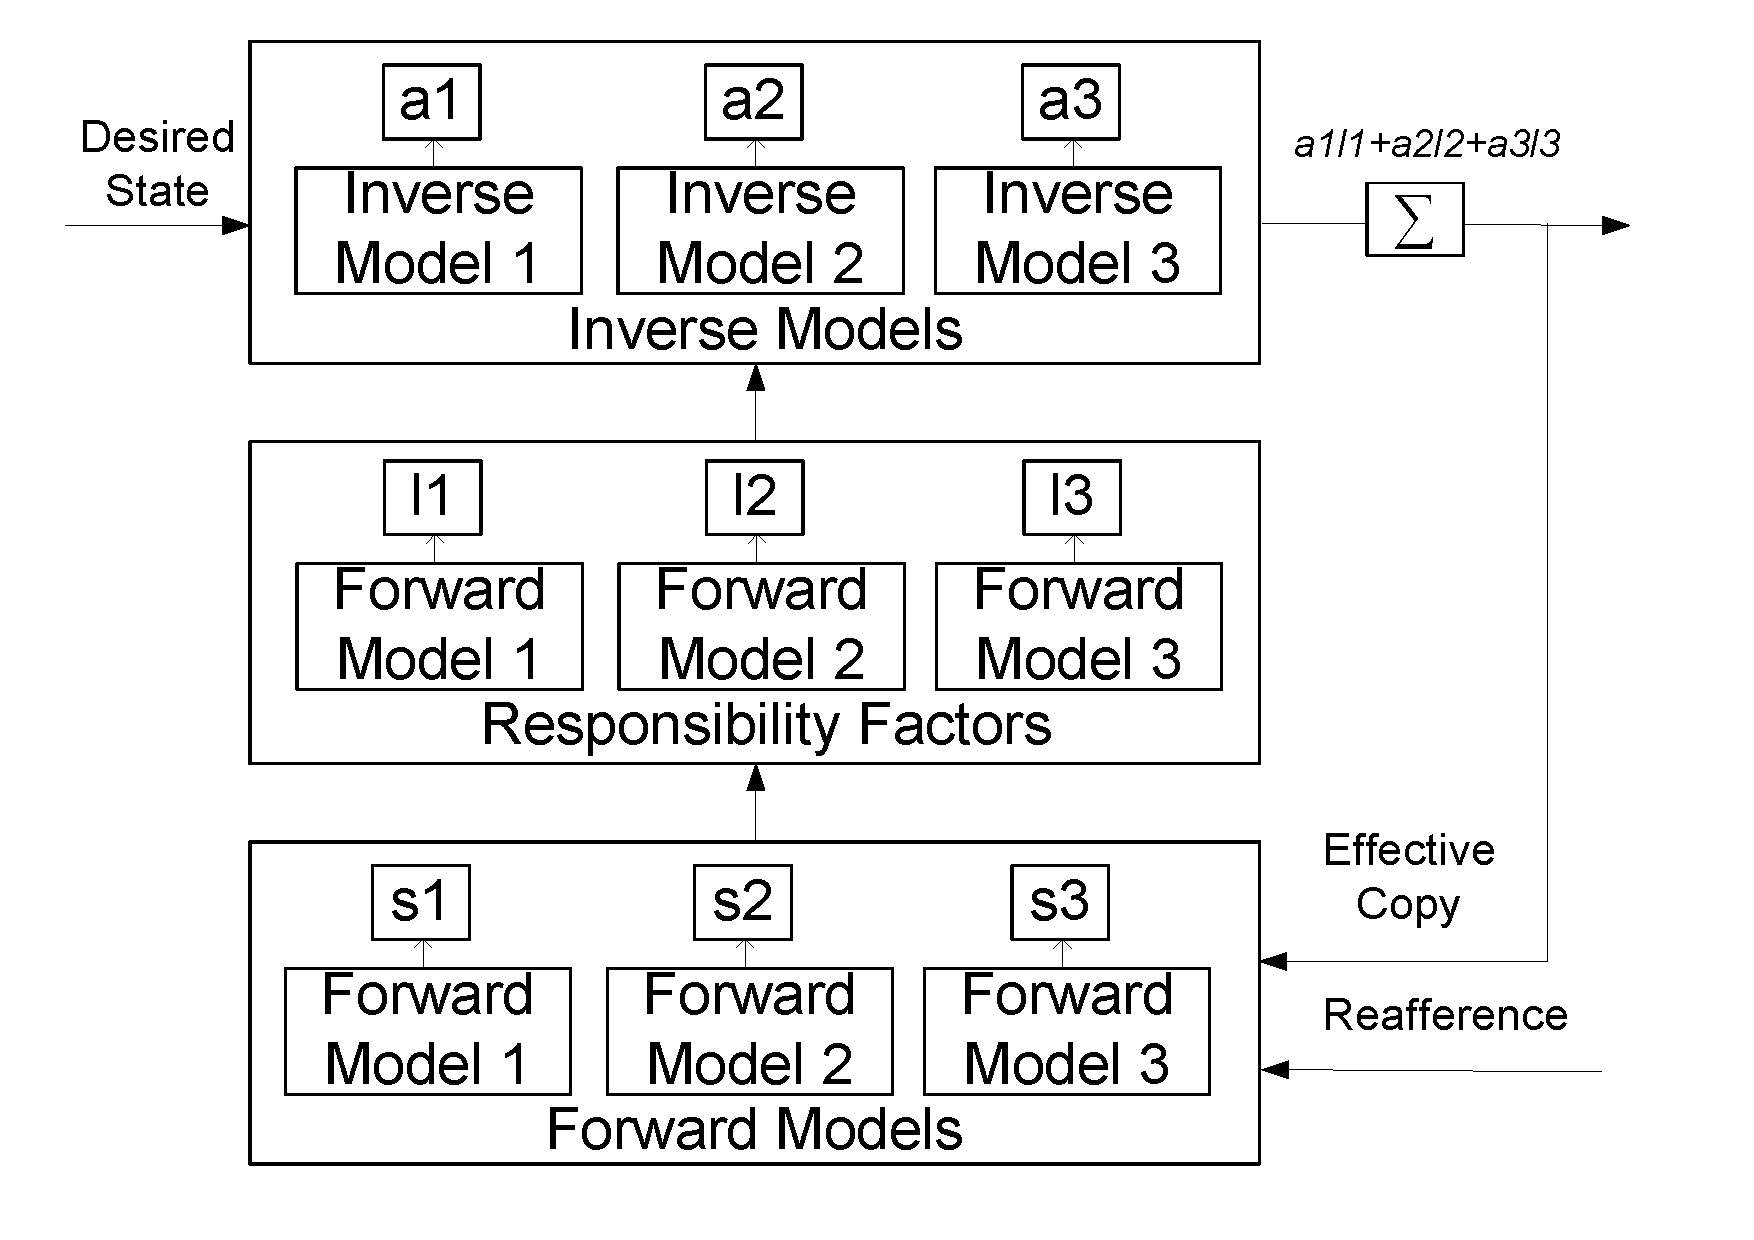
\includegraphics[width=15cm]{./fig_cha4/control_3_2.pdf}}
  \caption{ \scriptsize{Control flow diagram of forward-inverse model in motor control. (a) System overview. Pairs of forward and inverse models work together to generate final motor command. The mechanism inside the red box is shown underneath. (b) A example of a 3 modules model. The forward models predict current task context (s1, s2, s3) and estimate the accuracy of their prediction (l1, l2, l3). These accuracy is called ``Responsibility Factors'' as they decide how much responsibility each inverse model should take in the final command. The Inverse models generate commands (a1, a2, a3) and the final command is the summation of them factorized by their responsibility factor (a1l1+a2l2+a3l3).  }
}
\label{fig:control}
\end{figure}

% ----------- One model for both -------------
%The internal model ${\Omega})$ (forward model and inverse model) is encoded by the joint distributions of the variables, i.e. $p(s_t,s_{t+1},a_{t-1},a_t\mid{\Omega})$. This joint distribution encodes the forward model and the inverse model at the same time and both of their functionalities can be realized by the Gaussian Mixture Regression (GMR). For a given previous state and previous motor command, GMR provides a close-form solution to compute the anticipating state $s_t$, i.e. $p(s_{t+1}{\mid}s_{t},a_{t},{\Omega})$. For a given current state and desired state, we can compute the motor command using GMR, i.e. $p(a_t{\mid}s_t,s^{*}_{t+1},{\Omega_f})$. In some tasks, the initial status of the system remains unchanged for a certain time until the exert force or torque is big enough to change it. This will cause degeneracy in the inverse model. To solve this problem we include the previous motor command into the model, i.e. $p(a_t{\mid}s_t,s^{*}_{t+1},a_{t-1},{\Omega_f})$.

% --------- one model for each ----------
The forward model $\Omega_I$ is encoded by the joint distributions of the current system state, previous system state and the previous motor command, i.e. $p(s_t,s_{t-1},a_{t-1}\mid{\Omega_I})$. For a given object displacement and a motor command, the Gaussian Mixture Regression (GMR) provides a close-form solution to compute the anticipating object displacement $s_t$, i.e. $E(s_t{\mid}s_{t-1},a_{t-1},{\Omega_I})$. The inverse model $\Omega_f$ is encoded by the joint distributions of the current object displacement $s_t$ and the desired object displacement $s^{*}_{t+1}$. In some tasks, the initial status of the system remains unchanged for a certain time until the exert force or torque is big enough to change it. This will cause degeneracy in the inverse model. To solve this problem we include the previous motor command into the model, i.e. $p(s_t,s^{*}_{t+1},a_{t-1},a_t{\mid}{\Omega_F})$.



% Non-linear, multi model. What to solve in multi model
%As discussed above, one of the characteristics of manipulation task is the changing kinematics and dynamics configuration.
%In different task contexts, the pattern of the correlation between the displacement and action may be different.
By clustering the training data into different groups as discussed in Section~\ref{cha4:sec2:learn:cluster}, we are able to discover the number of different patterns, i.e. number of modules. We train one GMM on each of the modules to encode the different changing patterns of the task context.


% Learn system dynamics, impedance, admittance.

%Phases
%A single model is usually not enough to encode all these different configurations. Therefore we adopt a multiple modular approach to model the different environment. There are two key problems needed to be resolve in a multiple modular approach: how many models to build (Section~\ref{cluster}) and how to weight the models during the control process (Section~\ref{rf}).




\subsection{Multiple modular adaptive control}
\label{cha4:sec2:control}
%% forward-inverse modeling
%%After clustering the data into different groups, we train each cluster with the GMM $p(X_T, X_{t+1}, U_{t-1}, U_t {\mid} {\Omega})$.
%We model each of the cluster to encode the human control policy under different dynamics.
%Neuroscientists suggested that human use a mixture of forward model and inverse model for motor control. The forward model
%With the learned multiple models, we adopt the MOSAIC~\cite{haruno2001mosaic} architecture to control the system. The basic concept of MOSAIC is that the human brain use multiple inverse models to control the system, which is augmented with a forward models. In human brain there exist multiple pairs of coupled forward and inverse models. The forward models estimate the reliability of the inverse model in the current context, and the final motor command is a linear combination of all the commands from the inverse models.
%In object manipulation, the system dynamics can be rapidly changing over time and we need more than one model to describe it. Our learnt multiple GMMs are used to describe the system in these different contents. First we need to infer the behavior of the system. Having deduced this information, we need to decide how to manipulate the system.

Once the number of modules is found and the multiple pair of forward and inverse models are learnt, they are used to compute motor commands for task execution.
We consider the human motor system acts upon by motor command $a_t$ at time $t$ with current system status $s_t$. The resulting system status at time $t+1$ then is

\begin{equation}
\label{equ:e1}
s_{t+1} = f\left(s_t,a_t\right)
\end{equation}

The goal of the controller is to generate a motor command that bring the current system status from $s_t$ a desired state $s^*_{t+1}$:

\begin{equation}
\label{equ:e2}
a_t = g\left({s^*_{t+1},s_t}\right)
\end{equation}

According to the discussion in Section~\ref{cha4:sec2:learn:model}, equation~\ref{equ:e1} represents the forward model and equation~\ref{equ:e2} represents the inverse model. It takes three steps to compute the motor command $a_t$:
\begin{enumerate}
\item Compute expected system state $\hat{s}_t$ by each forward model
\item compute responsibility factor $\lambda$ for each module
\item Compute motor command by each inverse model and compute the final motor command $a_t$
\end{enumerate}


\subsubsection{Anticipate sensory output by forward model}
\label{cha4:sec2:control:forward}
With the $k$-th forward model we can estimate the current status $\hat{s}_t$ by
\begin{equation}
\label{equ:e3}
\hat{s}^k_{t} = E\left({s_{t-1}, a_{t-1} \mid \Omega^k_I}\right)
\end{equation}

%and
%
%\begin{equation}
%\label{e4}
%u^i_t = E\left({x^*_{t+1},x_t, u^i_{t-1} \mid \Omega^i}\right)
%\end{equation}

%These two equations will be described later in details.
This equation is to predict the environment status based on the observation and prediction on the controller's influence on the system. The expectation values of the current system status of the $k$-th module is computed by the $Gaussian$ $Mixture$ $Regression$ (GMR). The computation is as follow.

With the sensory input $\{s_{t-1},a_{t-1}\}$ as a query point $q$ we define:

\begin{equation}
{
 {\mu}_{q,n}^k = \begin{pmatrix} {\mu}_{s_{t-1},n}^k    \\
                                        {\mu}_{a_{t-1},n}^k
                        \end{pmatrix}
}
\end{equation}
\begin{equation}
{
{\Sigma}_{qq,n}^k =  \begin{pmatrix} {\Sigma}_{s_{t-1}s_{t-1},n}^k  & {\Sigma}_{s_{t-1}{a_{t-1},n}}^k  \\
                                            {\Sigma}_{{a_{t-1}}{s_{t-1}},n}^k  & {\Sigma}_{{a_{t-1}}{a_{t-1}},n}^k
                            \end{pmatrix}
}
\end{equation}
and GMR then uses:

\begin{equation}
{
\hat{\mu}_{s_t,n}^k = {\mu}_{s_t,n}^k + \Sigma_{{s_t}q,n}^k({\Sigma}_{qq,n}^k)^{-1}(q-{\mu}_{q,n}^k)
}
\end{equation}

\begin{equation}
{
\hat{\Sigma}_{{s_t}{s_t},n}^k = {\Sigma}_{{s_t}{s_t},n}^k - {\Sigma}_{{s_t}q,n}^k({\Sigma}_{qq,n}^k)^{-1}{\Sigma}_{q{s_t},n}^k
}
\end{equation}


Finally, all the $N$ Gaussian components of the $k$-th module\footnote{Different modules may have different number of Gaussian components.} are taken into account and the current sensory data $\hat{s}_t$ is predicted as the mean $\hat{\mu}_{s_t}$ with the covariance $\hat{\Sigma}_{s_t,s_t}$ according to:

\begin{equation}
{
\hat{\mu}_{s_t} = \sum_{n=1}^N{\beta_n(q)}\hat{\mu}_{s_t,n}^k
}
\end{equation}
\begin{equation}
{
\hat{\Sigma}_{{s_t}{s_t},n} = \sum_{n=1}^N{\beta_n(q)}^2\hat{\Sigma}_{{s_t}{s_t},n}^k
}
\end{equation}
where
\begin{equation}
{
\beta_n(q) = \frac{p_{n}p(q|{\mu}_{q,n}^k,{\Sigma}_{qq,n}^k)}
{\sum_{n=1}^N{p_n}p(q|{\mu}_{q,n}^k,{\Sigma}_{qq,n}^k)}
}
\end{equation}



\subsubsection{Weight modules by responsibility factor}
\label{cha4:sec2:control:rf}

In a multi-module approach, choosing the proper modules to compute the motor command is crucial. For this we rely on the computation of the responsibility factor. The responsibility factors act as the weight of the modules. Each module has its responsibility factor at every time step, the final motor command at that time step is the linear combination of the commands generated from each module multiplied by their responsibility factors.
The responsibility factor is a measurement of the reliability of using one model to represent the current system context.
%The measurement is computed by the discrepancy between the anticipating current system state $s_t$ of the forward model and the actual current system state $s'_t$ from the sensory feedback:
%
%\begin{equation}
%\lambda'^j_t = {$s'_t$ - p(s_t{\mid}s_{t-1},a_{t-1},\Omega^j)}}
%\end{equation}
%
%where $n$ is the number of models.

As the models are built as GMMs, it is easy to estimate the likelihood of one data point belongs to a particular module. The actual current state from the sensory feedback, the previous state and the previous motor command forms a query point $\{s_t,s_{t-1},a_{t-1}\}$. The responsibility is computed by the likelihood of the current query data point in each module, normalized by the total sum:

\begin{equation}
\lambda^j_t = \frac{p(s_t,s_{t-1},a_{t-1}\mid \Omega_I^j)}{\sum_{k=1}^{K}{p(s_t,s_{t-1},a_{t-1}\mid \Omega_I^k)}}
\end{equation}
where $K$ is the number of modules.

%Note the forward model is embedded in this computation of the responsibility factor. The likelihood of the query point $p(s_t,s_{t-1},a_{t-1}\mid \Omega^j$ in the $j-th$ module is equivalent to the discrepancy between the expected current system state $s_t$ of the forward model and the actual current system state $s'_t$ from the sensory feedback, factorized by the variance of the forward model.

\subsubsection{Generate motor command by Inverse Model}
\label{cha4:sec2:control:inverse}
%While the forward models predict the current status of the system by the previous status and motor commands, the inverse models generate the next motor command according to the current status and the next target status. In reality, given a current state and a desired state, the command bring the robot to the desired state is not unique. In addition, during object manipulation, it is often the case that the force applying on the object various but the object position does not change because of friction. Therefore we include the previous command into the query point in order to generate the next command without redundance. Hence the command generated by each model is computed by equation~\ref{e4}.
%\subsubsection{Mix of Model}
%\label{mix}

The motor command $a^k_t$ for the $i$-th inverse model is computed by GMR with the same steps  described in Section~\ref{cha4:sec2:control:forward}. The responsibility factors $\lambda^j$ act as the weights of each model in the control system. The higher the responsibility is, the more response the model takes in the control system. Therefore, the final motor command generated by this multiple model system is

\begin{equation}
\label{equ:e_mix}
s_t = \sum_{k=1}^K{\lambda^k a_t^k} = \sum_{k=1}^K{\lambda^k E\left({s^*_{t+1},s_t, a^k_{t-1} \mid \Omega^k_I}\right)}
\end{equation}

These three steps are computed with a close form solution. This ensures that this system can react quickly to the changes in the environment by adjusting the responsibility factor.



